\documentclass[letterpaper,10pt,conference]{ieeeconf}
\IEEEoverridecommandlockouts
\overrideIEEEmargins
\usepackage{fontspec}
\setmainfont{Times New Roman}\setsansfont{Arial}\setmonofont{Menlo}
\usepackage{amsmath,amssymb,graphicx,booktabs,cite,url}
\graphicspath{{figures/}}
\newcommand{\vct}[1]{\vec{#1}}
\newcommand{\BudgetSpeed}{$0.283\,\mathrm{m/s}$}
\newcommand{\WalkSpeed}{$0.126\,\mathrm{m/s}$}
\newcommand{\AbstractRateResult}{The maximum sector-command rate decreases from 1517 to 536 degree/s relative to the original allocator, retaining 99.95\% of its mean forward speed.}

\title{\LARGE\bf Rewind-Aware Rolling Allocation\\for an Articulated Arc-Leg Hexapod}
\author{\mbox{}}
\begin{document}
\maketitle\thispagestyle{empty}\pagestyle{empty}
\begin{abstract}
A finite-arc leg with bounded distal rotation must periodically rewind its rolling motion. A geometric excursion limit alone can leave insufficient swing time for a rate-bounded rewind. We present a rolling allocator that couples available swing time, the next reindexing opportunity, and residual travel assigned to articulation. In a 268-trial MuJoCo mechanism study, it reduces the largest sector-command rate from 1517 to 536 degree/s while retaining 99.95\% of the original allocator's mean forward speed. The sector bound does not constrain the summed joint target. We therefore conduct 176 additional trials with a common all-joint target governor, longer horizons, and changing commands. All 128 rate-limited trials satisfy the issued-target and inner-setpoint bounds. At a 0.45 m/s command and 80\% of nominal no-load speed limits, the proposed allocator achieves 0.227 m/s when its gait clock waits for target issuance and 0.316 m/s with a fixed clock, against 0.289 m/s without the governor. The fixed clock changes the requested trajectory, while periodic reindexing remains competitive throughout. These results establish command-level bounds and quantify their tracking tradeoffs; they do not establish loaded actuator feasibility or an advantage for adaptive scheduling.
\end{abstract}

\section{INTRODUCTION}
An articulated leg ending in a finite circular arc can move through both rolling and joint articulation. With a bounded distal joint, the arc eventually reaches an orientation from which it must be lifted and rewound. The controller must therefore reserve enough swing time to restore the arc before its next stance. This constraint matters even when the robot moves successfully: a rewind without an explicit rate constraint may preserve body speed while demanding abrupt distal motion.

The relevant limit is temporal as well as geometric. At a swing duration of 0.20 s and a sector-rate budget of $540^\circ$/s, a rest-to-rest quintic rewind can recover only $57.6^\circ$, despite a geometric excursion of $100^\circ$. Figure~\ref{fig:overview} illustrates this mismatch and the measured effect of limiting rewind demand. Reducing the allowed rotation also changes how much contact travel the articulated joints must supply. A sector bound can consequently make a previously reachable stance trajectory infeasible unless the controller also schedules reindexing and reallocates the residual travel.

We couple these decisions in a position-target allocator. It assigns rolling roles from contact geometry, constrains sector excursion using swing time, reindexes before the next opportunity would be missed, and subtracts the realized rolling increment from the requested articulated motion. The analytical component is a sufficient sector-command bound for a specified interpolation profile. We first test the transport cost of this sector constraint, then test the summed joint commands under a common rate governor. The second comparison exposes the effect of retiming the gait versus allowing the requested trajectory to change.

Our contributions are: (1) a swing-time constraint coupled to post-saturation contact-travel allocation, including an explicit statement of the sector-rate guarantee and its assumptions; and (2) a paired mechanism study that compares the complete rewind treatment with the original allocator, periodic reindexing, and component restrictions under one morphology. The study includes all-joint rate limits, command transitions, and 60 s trials. A concavity-preserving collision approximation supports the experiments. Curved legs, stride-level rolling/stepping, quintic interpolation, convex decomposition, and the added target governor are established tools, not separate novelty claims.

\begin{figure}[t]
\centering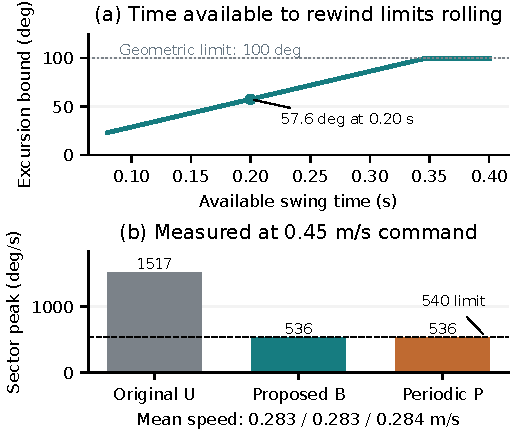
\includegraphics[width=\columnwidth]{overview.pdf}
\caption{The rewind constraint and its measured effect. (a) Analytical excursion bound for $\Omega=540^\circ$/s and a $100^\circ$ geometric limit. (b) Largest sector rates over eight initial phases; speeds are eight-trial means. U, B, and P all complete the 8 s trials. P shows that periodic reindexing is a competitive alternative. The dashed rate bound applies to the sector component only.}
\label{fig:overview}
\end{figure}

\section{RELATED WORK}
RHex established the mobility of a hexapod with continuously rotating compliant curved legs~\cite{saranli2001rhex}. Q-Whex further develops quasi-wheeled hexapod motion~\cite{zhang2023qwhex}. Energy-oriented design guidelines and kinematic studies also connect C-leg geometry to locomotion performance~\cite{vina2021cleg,burzynski2024kinematics}. These systems motivate efficient use of curved contacts, while the present problem concerns an arc mounted after two additional articulated joints and restricted to a bounded position range.

Transformable leg-wheel robots provide the closest morphological context. Quattroped shares actuation across wheel and leg configurations~\cite{chen2014quattroped}, and TurboQuad addresses smooth behavioral transitions~\cite{chen2017turboquad}. R-Taichi studies rolling and swing strategies on a transformable two-degree-of-freedom limb, including physical experiments~\cite{xue2025rolling}. Chang and Lin describe stride-level hybrid locomotion with aerial repositioning and energy-oriented optimization~\cite{chang2026stride}. Accordingly, combining rolling and swing within a stride is established. Our narrower question is how to bound the rotation of a fixed finite sector by its available rewind interval and allocate the remaining contact travel to articulation.

Articulated wheel-leg platforms also coordinate contact placement and rolling, including ASTERISK H~\cite{yoshioka2008asterisk}, whole-body wheeled-quadruped control~\cite{bjelonic2019keep}, and online gait-sequence generation with model predictive control~\cite{bjelonic2021wholebody}. These methods address broader force and motion planning problems. Our allocator uses geometric roles and position targets without online force optimization or learned policies. The experiments therefore test its internal mechanisms under a common embodiment and motor setup, rather than claim superiority over whole-body controllers on different robots.

Mane and Hubicki~\cite{mane2024rolling} derive rolling constraints and augmented dynamics for smooth planar body and terrain curves, assuming single-point no-slip contact. Our contact-travel allocator uses an instantaneous axis tangent and allows simulated slip; it is not a replacement for their curved-terrain dynamics model. The present question concerns finite-sector rewind and target issuance across successive contacts.

Repeatable testing matters when small control changes alter contact sequences. Weng et al.~\cite{weng2024testing} demonstrate the importance of controlled conditions in legged-robot evaluation. We use fixed paired phases and explicit parameter stress conditions, report failures as well as transport, and distinguish these deterministic comparisons from hardware reliability estimates.

\section{PLATFORM AND CONTACT REPRESENTATION}
\subsection{Embodiment and Actuation}
The model is a hexapod with three revolute joints per leg and eighteen actuators. The first joint steers the limb about a vertical axis. The second and third joints articulate the leg, with the third joint also rotating the arc; there is no additional wheel actuator. The model mass is 4.161 kg. The tire envelope has an outer radius of 122.5 mm, an inner radius of 112.5 mm, and a width of 44 mm. Dimensions in the historical drawing provide manufacturing context but do not calibrate the compliance of the simulated tire.

Every condition uses the same floating base, inertias, controller gains, voltage limits, and nominal pose. The actuator path computes a proportional-derivative torque request and a bounded voltage command,
\begin{align}
 \tau_j^c&=k_{p,j}(q_j^\star-q_j)+k_{d,j}(\dot q_j^\star-\dot q_j),\\
 V_j&=\operatorname{sat}_{[-12,12]}[(R_j/K_j)\tau_j^c+K_j\dot q_j].
\end{align}
Reflected rotor inertia is included. The baseline gait setup disables the additional target-profile velocity and acceleration limits and doubles the middle-joint proportional gain, with damping scaled by $\sqrt{2}$. The additional all-joint study explicitly reinstates velocity profile limits. Voltage and torque limits remain active in both studies; neither setup identifies loaded actuator capability.

\begin{figure}[t]
\centering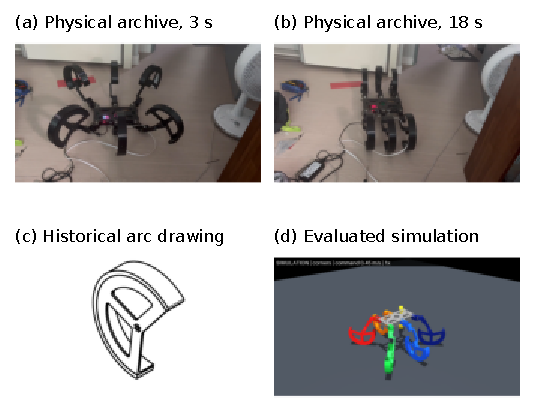
\includegraphics[width=\columnwidth]{platform.pdf}
\caption{SCONE embodiment and evaluated model. (a,b) Archival floor-motion frames at source times 3 and 18 s. (c) Historical arc fabrication drawing. (d) Nominal simulation pose. The physical clips use an undocumented earlier controller and include external cables; they do not validate the proposed allocator on hardware.}
\label{fig:platform}
\end{figure}

\subsection{Contact Geometry and Rolling Direction}
Let $\vct{a}_i$ be the distal axis, $\vct{o}_i$ a point on it, and $\vct{p}_{c,i}$ the geometric support centroid. The planar material velocity induced by unit distal rotation is
\begin{equation}
 \vct{t}_i=\vct{a}_i\times(\vct{p}_{c,i}-\vct{o}_i),\qquad
 r_i=\|\vct{t}_{i,xy}\|.\label{eq:tangent}
\end{equation}
The geometric lowest point can remain almost stationary while successive material points move through contact. Its finite difference therefore does not identify the rolling direction. We instead use the axis-based tangent in~\eqref{eq:tangent}.

A geometric scan of the nominal standard pose gives usable sector offsets of $[-100^\circ,100^\circ]$ after margins. Across six legs and 21 offsets per leg, the lowest-patch centroid changes by at most 2.828 mm horizontally and 0.053 mm vertically. The centroid includes mesh vertices within 0.1 mm of the minimum height. This geometric check motivates adding a sector offset to an articulated IK solution, subject to the limits of a rigid contact approximation.

\subsection{Preserving the Inner Cavity}
Ordinary MuJoCo mesh collision uses a convex representation~\cite{mujococollision}. One mesh per tire therefore fills its annular interior, despite rendering an open arc. We replace the active tire contact by a union of convex parts generated with CoACD~\cite{wei2022coacd}. The original mesh remains visual geometry, and explicit body mass and inertia are unchanged. CoACD 1.0.14 uses a 2 mm real-metric concavity threshold and a fixed seed, yielding 24 parts per tire.

An independent probe places a sphere of radius 1 mm at the axle center. The single-hull representation reports contact at approximately $-23$ mm signed distance; the decomposition reports no contact. Over 720 planar directions, the change in the support function is below 0.004 mm. The summed convex-part volume exceeds the original mesh volume by 2.76\%, so the representation remains approximate. These checks verify a preserved cavity and essentially unchanged outer-plane support, rather than exact reproduction of all concave collisions or soft-tire deformation.

\begin{figure}[t]
\centering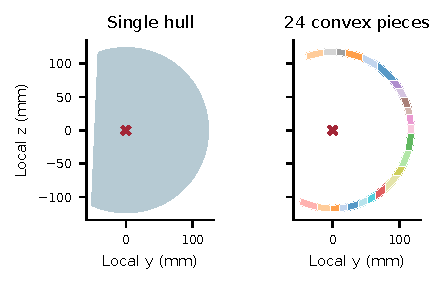
\includegraphics[width=\columnwidth]{collision.pdf}
\caption{Tire collision cross-section from actual mesh data. The single hull (left) fills the cavity. The 24-piece approximation (right) leaves the axle-center probe free while preserving the outer support envelope. Colors distinguish convex pieces; both models retain the same inertial properties.}
\label{fig:collision}
\end{figure}

\section{REWIND-BUDGETED TRAVEL ALLOCATION}
\subsection{Steering and Contact Roles}
For a filtered body command $\vct{c}=[v_x,v_y,\omega_z]^\top$, the required contact travel in the body frame is
\begin{equation}
 \vct{u}_i=-[v_x-\omega_z y_i,\ v_y+\omega_z x_i]^\top,\label{eq:travel}
\end{equation}
where $[x_i,y_i]^\top$ is the nominal contact relative to the footprint centroid. We evaluate both distal rotation signs, clip steering to $\pm35^\circ$, and choose the direction $\hat{\vct{d}}_i$ with greatest alignment to $\vct{u}_i$. A leg qualifies for rolling when the alignment is at least 0.70; fewer than two qualifying legs causes an all-stepping assignment. Under forward motion, this geometry selects legs $\{1,2,5,6\}$ to roll while $\{3,4\}$ step (Fig.~\ref{fig:concept}).

\begin{figure}[t]
\centering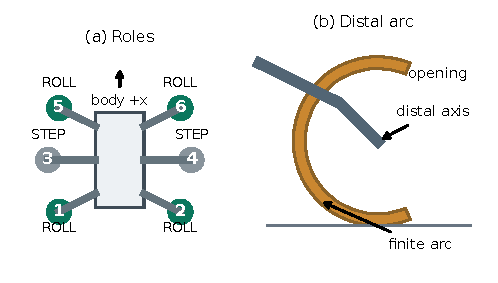
\includegraphics[width=\columnwidth]{concept.pdf}
\caption{Role allocation and finite distal arc, shown schematically. The upper joint changes both rolling heading and foot location. Roles and steering are therefore latched at lift-off. IDs follow the model convention.}
\label{fig:concept}
\end{figure}

\subsection{Rewind Distance and Sector-Rate Bound}
The alternating tripods $\{1,4,5\}$ and $\{2,3,6\}$ have phase offsets of one half-cycle. Frequency $f$ and duty factor $D$ give a swing duration $T_s=(1-D)/f$. A sector rewind from $\theta_{\rm lo}$ to a fixed home $h_i$ uses
\begin{equation}
 \theta(s)=\theta_{\rm lo}+S(s)(h_i-\theta_{\rm lo}),\quad
 S(s)=10s^3-15s^4+6s^5,
\end{equation}
with $s\in[0,1]$. Since $S'(s)=30s^2(1-s)^2$ has maximum $15/8$, a complete swing satisfies $|\dot\theta|\le\Omega$ if
\begin{equation}
 |\theta_{\rm lo}-h_i|\le B,\qquad B=\frac{8}{15}\Omega T_s.\label{eq:budget}
\end{equation}
For $f=2$ Hz, $D=0.60$, and $\Omega=540^\circ$/s, the rewind budget is $B=57.6^\circ$. This is smaller than the geometrically available sector excursion. We use $h_i=0$, which lies in every evaluated sector interval.

During stance, the next sector target is projected into the intersection of its geometric interval and rewind budget:
\begin{equation}
 \theta_{i,k+1}=\Pi_{[\ell_i,u_i]\cap[h_i-B,h_i+B]}
     (\theta_{i,k}+\Delta t\,\omega_{i,k}).\label{eq:project}
\end{equation}
The proposed rate $\omega_{i,k}$ is itself bounded by $\Omega$. For a state already in this interval, projection cannot increase the step magnitude beyond $\Omega\Delta t$. Thus stance respects both the excursion and discrete rate bounds. In swing, we apply an additional projection onto $[\theta_{i,k}-\Omega\Delta t,\theta_{i,k}+\Omega\Delta t]$. This slew guard preserves the discrete sector-rate invariant even when a swing is interrupted or resumed. The complete-swing premise in~\eqref{eq:budget} is required for reaching home within $T_s$; the slew guard alone does not guarantee that endpoint under interruptions.

The budget in~\eqref{eq:budget} is specific to the selected quintic profile, not the maximum recoverable angle for every trajectory. A constant-speed return would have a different factor and different endpoint smoothness. For a geometric reserve $A_i$ about home, the usable excursion is $\min(A_i,B)$. Thus the temporal constraint becomes active when $15A_i/(8\Omega T_s)>1$. This criterion describes where a geometric limit is insufficient; it does not prove contact stability or IK reachability.

A rolling leg decides whether to reindex at swing-window entry, based on spent reserve, loss of alignment, or predicted exhaustion before its next opportunity. For a locally constant sector rate, skipping the current window predicts $\theta_i^+=\theta_i+\omega_i/f$. If this value lies outside the intersection in~\eqref{eq:project}, the leg reindexes now. This one-cycle lookahead is a scheduling heuristic under changing commands, while the excursion and slew bounds remain explicit. This avoids starting a quintic trajectory midway through its allotted window. Roles are updated at actual lift-off. A stepping leg uses every swing window; rolling legs can skip unneeded swings. The schedule leaves at least three legs commanded in stance, while the number of loaded contacts is measured separately.

\subsection{Allocation After Saturation}
Before angular projection, the requested rolling speed is the projection of contact travel onto the steered rolling direction, scaled by an authority $\beta_i$. Authority fades over the last $12^\circ$ of the geometric interval. After~\eqref{eq:project}, articulation receives the residual based on the increment that will actually be commanded:
\begin{equation}
 \vct{u}^{\rm art}_i=\vct{u}_i-
 s_i r_i\frac{\theta_{i,k+1}-\theta_{i,k}}{\Delta t}\hat{\vct{d}}_i,\label{eq:residual}
\end{equation}
where $s_i$ maps the selected motor sign to rolling direction. This subtraction prevents the walking trajectory from requesting travel already assigned to rotation. Using the pre-saturation request would leave an unaccounted residual once the rewind budget is exhausted.

The residual is integrated into a stance offset, bounded by a 90/70 mm longitudinal/lateral elliptical workspace. Numerical IK generates articulated targets with a $40^\circ$ distal-branch guard and stride backoff when needed. The sector offset is added to the distal target, and final targets are clipped to $[0^\circ,360^\circ]$. The allocation equality describes commanded kinematics before workspace and final motor clipping; tracking lag and slip need not satisfy it. In particular, the summed distal target contains both IK and sector motion. The sector-rate invariant is not a bound on that sum. Before final clipping, $q^\star_{3,i}=q^{\rm IK}_{3,i}+\theta_i$. A physical target-rate constraint would require
\begin{equation}
 |\Delta q^{\rm IK}_{3,i}+\Delta\theta_i|\le\dot q_{3,i}^{\max}\Delta t.\label{eq:joint}
\end{equation}
A sufficient bound is $|\Delta q^{\rm IK}_{3,i}|+|\Delta\theta_i|\le\dot q_{3,i}^{\max}\Delta t$. The allocator alone does not enforce this coupled constraint. The common governor below limits the complete issued target and measures the resulting tracking cost.



\subsection{All-Joint Target Governor}
A sector bound alone does not enforce~\eqref{eq:joint}. We therefore add a common, simulation-only governor after summing IK and sector motion, and compare U, B, and P through the same governor. This conventional rate-limiting construction is a feasibility probe, not an additional novelty claim.

Let $n_j$ and $n_j^d$ be the issued and desired integer motor positions, with resolution $\delta=360^\circ/4096$. For joint-rate limit $L_j$, define $C_j=\lfloor L_j\Delta t/\delta\rfloor$ and $d_j=n_j^d-n_j$. At each wall-clock update,
\begin{align}
 \alpha&=\min\!\left(1,\min_{j:d_j\ne0}\frac{C_j}{|d_j|}\right),\\
 n_j^+&=n_j+\operatorname{sgn}(d_j)\lfloor\alpha|d_j|\rfloor.\label{eq:governor}
\end{align}
If all $d_j=0$, we set $\alpha=1$. All tested $C_j$ are positive. Thus $\delta|n_j^+-n_j|/\Delta t\le L_j$ for all eighteen joints, including the first measurement command. We also cap the inner motor profile at or below $L_j$, using its discrete speed units. Otherwise, a bounded 20 ms goal step could still produce a larger 2 ms internal setpoint rate. These bounds apply to commands, not measured joint motion, acceleration, or contact feasibility.

The model maps proximal, middle, and distal joints to MX-28, XM430-W350, and XM430-W210 actuators. Their published 12 V no-load speeds are 55, 46, and 77 rpm~\cite{robotisMX,robotisW350,robotisW210}, giving $L^0=(330,276,462)^\circ$/s by joint group. We test $L=\rho L^0$ for $\rho=1.0,0.8,0.5$. These are declared stress levels anchored to nominal motor data, not measured loaded capabilities or uncertainty distributions.

In the fixed-clock mode F, the gait advances every 20 ms even when the issued target lags. In the governed-clock mode H, the next gait step is requested only after the preceding quantized target has been fully issued. H preserves the target order and retimes the gait and its command filter together; it does not wait for measured joint convergence. External commands remain functions of wall time, so this retiming can introduce tracking delay. All comparison controllers use identical clock and profile settings.


\section{EXPERIMENTAL METHOD}
\subsection{Baseline Mechanism Study}
We use MuJoCo 3.10.0~\cite{todorov2012mujoco}, a 2 ms physics step, and a 20 ms command update. Each fresh model is initialized, placed at the common nominal pose, and settled for 1 s. The 0.15 s command filter and initial role-adoption transient are included. The maximum step height is 25 mm. No settings are retuned between comparison controllers.

The first study measures 8 s per trial. Its main matrix tests seven conditions (Table~\ref{tab:conditions}), two forward commands (0.18 and 0.45 m/s), and eight phases $k/8$, giving 112 trials. U is the original allocator; B adds the swing-time budget, fixed home, next-window lookahead, and slew guard together. This contrast tests the complete rewind treatment, not an isolated projection operator.

\begin{table}[t]\centering\small
\caption{Controller restrictions in the mechanism study}
\label{tab:conditions}
\begin{tabular}{cp{6.7cm}}\toprule
Code & Definition\\\midrule
U & Original allocation with geometric sector limits.\\
B & Rewind-budgeted allocation with next-window lookahead.\\
G & B without the next-window budget lookahead.\\
N & B with all rolling roles disabled.\\
S & B without subtracting realized rolling travel.\\
D & B with rolling-leg reindexing disabled after adoption.\\
P & Periodic rolling-leg swings at every opportunity.\\\bottomrule
\end{tabular}\end{table}

Additional B/N/S trials cover seven constant commands over four phases: forward 0.30 m/s, reverse $-0.18$ m/s, lateral $\pm0.12$ m/s, yaw $\pm0.45$ rad/s, and a curve at 0.18 m/s with 0.35 rad/s yaw (84 trials). Separate mass $\times1.2$, friction $\times0.5$, and actuator-strength $\times0.8$ cases add 36 high-command trials. Single-hull contacts at both forward commands add 24; physics steps of 1 and 4 ms add 12. These declared numerical stress cases are not hardware uncertainty distributions. The baseline study totals 268 trials.

\begin{table*}[t]\centering\small
\caption{Baseline main matrix: eight phases and 8 s windows}
\label{tab:main}
\begin{tabular}{ccccccc}\toprule
 & \multicolumn{2}{c}{0.18 m/s command} & \multicolumn{2}{c}{0.45 m/s command} & \multicolumn{2}{c}{High-command peak ($^\circ$/s)}\\
Code & Complete & Mean speed & Complete & Mean speed & Sector & Total distal\\\midrule
U & 8/8 & 0.114 & 8/8 & 0.283 & 1516.8 & 3299.5\\
B & 8/8 & 0.114 & 8/8 & 0.283 & 536.4 & 1405.5\\
G & 8/8 & 0.114 & 0/8 & -- & 535.7 & 1291.9\\
N & 8/8 & 0.094 & 8/8 & 0.126 & 0.0 & 1763.2\\
S & 0/8 & -- & 0/8 & -- & 179.3 & 1301.6\\
D & 0/8 & -- & 0/8 & -- & 203.0 & 1291.9\\
P & 8/8 & 0.113 & 8/8 & 0.284 & 536.4 & 1191.8\\\bottomrule
\end{tabular}
\par\vspace{5pt}\noindent\parbox{.96\textwidth}{\footnotesize Speeds are m/s. At the high command, speed ranges are U [0.278,0.288], B [0.280,0.286], N [0.122,0.129], and P [0.281,0.285]. Total distal includes IK plus sector; it is not measured motor speed. Peaks of failed conditions cover only the interval before termination.}
\end{table*}

\subsection{Additional Joint-Limit Study}
We then freeze a separate 176-trial design, retaining the same model and allocator settings. New phases are $1/16,5/16,9/16,13/16$. U/B/P are compared under unlimited targets, H at $\rho=1.0$ and 0.8, and F at $\rho=0.8$. Both forward commands run for 20 s, yielding 96 trials. A stricter H setting of $\rho=0.5$ adds 12 high-command trials. The initial settled target, rather than measured joint position, initializes the governor.

Two 24 s sequences change commands every 6 s: forward 0.18, forward 0.45, stop, reverse $-0.18$ m/s; and forward 0.18 m/s, pure yaw 0.45 rad/s, curve $(0.18,0,0.35)$, forward 0.18 m/s. Unlimited and H at $\rho=0.8$ across all codes and phases give 48 trials. Twelve 60 s trials use both constant forward commands, all three codes, and phases $1/16$ and $9/16$ under H at $\rho=0.8$. Eight timestep checks repeat high-command B/P at these two phases with 1 or 4 ms steps.

Both designs fix source snapshots, model hashes, parameters, and output rules before their full runs. The second study follows the limitation identified in the first; it is not an independent external validation. Two short preflight runs check instrumentation and are excluded from all performance summaries. Every planned trial remains in the denominator. A rejected IK target, nonfinite state, or tilt exceeding $60^\circ$ terminates a trial. Completion requires the full prescribed horizon and is independent of tracking accuracy.

\subsection{Measurements and Interpretation}
Forward transport is net displacement along the initial chassis axis divided by duration. Velocity integration at the same root origin provides an independent check. For turning and reversing sequences, we emphasize body-frame translational and yaw-rate RMSE against the wall-clock command, rather than net forward displacement. Failed-trial speeds are not mixed with full-window averages.

The first study records sector rate and excursion, plus the summed distal-target rate from successive measurement commands. Its distal recorder omits the first command; that analysis is post hoc. The second study records all eighteen issued targets, including the first command, inner setpoint velocities, measured joint velocities, and issued-target tracking RMS. Requested-to-issued goal lag and the ratio of gait time to wall time distinguish trajectory alteration from clock delay.

Loaded-leg count uses distinct tire bodies with normal force above 1 N. Absolute mechanical work is $\int\sum_j|\tau_j\dot q_j|dt$, not battery energy. Slip integrates mean tangential velocity at loaded tire contacts; it depends on the contact manifold. Phase grids are deterministic, so we report means and observed ranges without population confidence intervals. Neither phase repetitions nor completion counts estimate field reliability.



\section{RESULTS}
\subsection{Baseline Mechanism and Its Limitation}
At the high command, B retains 99.95\% of U's mean speed and reduces the largest sector rate from 1516.8 to 536.4 degree/s (Table~\ref{tab:main}). U exceeds the 540 degree/s budget in every high-command trial; B has no violating frames. G rejects an IK target in all eight high-command trials, indicating that an excursion bound without next-window anticipation can leave an unreachable articulated residual. S and D reject targets in all main trials. These are failures of the specified restrictions and workspace, not universal results for those controller classes.

P attains comparable speed with a smaller largest distal-target rate than B. B's 1405.5 degree/s distal peak, although lower than U's 3299.5, still exceeds the sector budget. B uses 94.2 J of absolute joint work and 0.509 m integrated slip, compared with N's 58.1 J and 0.290 m; higher speed alone is not an efficiency result. Overall, 193/268 trials complete and all 75 terminations are rejected IK targets. B completes 68/68 with no sector violations, including the command and parameter cases. The original 1/2/4 ms check changes paired B/N speed by at most 0.00083 m/s; the geometry change gives at most 0.0123 m/s. These local results do not establish general robustness.

\begin{table*}[t]\centering\small
\caption{All-joint limit study at a 0.45 m/s command: four phases, 20 s per trial}
\label{tab:joint}\begin{tabular}{ccccccc}\toprule
 & & Speed (m/s) & $e_v$ (m/s) & Joint RMS ($^\circ$) & Goal lag ($^\circ$) & Clock fraction\\
Clock & Code & Mean [min, max] & Mean & Worst observed & Maximum & Mean\\\midrule
Unlimited & U & 0.287 [0.283, 0.291] & 0.188 & 19.38 & 0.0 & 1.000\\
Unlimited & B & 0.289 [0.285, 0.291] & 0.186 & 19.59 & 0.0 & 1.000\\
Unlimited & P & 0.289 [0.286, 0.291] & 0.186 & 19.45 & 0.0 & 1.000\\
\midrule
H, $\rho=1.0$ & U & 0.220 [0.218, 0.222] & 0.239 & 7.44 & 45.7 & 0.602\\
H, $\rho=1.0$ & B & 0.223 [0.219, 0.226] & 0.236 & 7.36 & 28.7 & 0.604\\
H, $\rho=1.0$ & P & 0.224 [0.220, 0.228] & 0.234 & 7.37 & 19.5 & 0.607\\
\midrule
H, $\rho=0.8$ & U & 0.231 [0.218, 0.244] & 0.232 & 5.58 & 47.5 & 0.566\\
H, $\rho=0.8$ & B & 0.227 [0.211, 0.241] & 0.235 & 5.54 & 30.0 & 0.552\\
H, $\rho=0.8$ & P & 0.228 [0.213, 0.242] & 0.234 & 5.56 & 20.8 & 0.555\\
\midrule
F, $\rho=0.8$ & U & 0.320 [0.315, 0.323] & 0.169 & 6.62 & 64.8 & 1.000\\
F, $\rho=0.8$ & B & 0.316 [0.309, 0.321] & 0.173 & 6.96 & 49.4 & 1.000\\
F, $\rho=0.8$ & P & 0.317 [0.309, 0.324] & 0.171 & 6.96 & 33.8 & 1.000\\
\bottomrule
\end{tabular}
\par\vspace{5pt}\noindent\parbox{.96\textwidth}{\footnotesize All entries complete 4/4 trials. H holds the gait clock until each goal is issued; F keeps the original gait clock. Joint RMS is the maximum, over trials and joints, of issued-target tracking RMS. Goal lag is requested minus issued target. Clock fraction is gait time divided by wall time. $\rho$ scales the joint-group no-load speeds; it is not a hardware confidence bound.}
\end{table*}

\begin{figure*}[t]\centering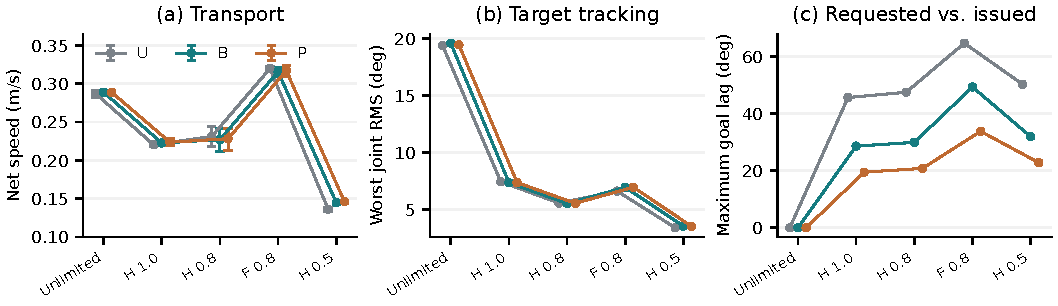
\includegraphics[width=.97\textwidth]{joint_limits.pdf}
\caption{High-command joint-limit comparisons. Speed markers and whiskers are four-phase means and ranges; tracking and goal-lag panels show worst observed values. H retimes the gait to issue every target; F keeps the original clock. H 0.5 belongs to the separately prescribed stricter-rate suite. All values include startup. The simple periodic P remains competitive.}
\label{fig:joint}\end{figure*}

\subsection{All-Joint Limits and Clock Choice}
All 176 additional trials complete their prescribed horizons. Every one of the 128 bounded trials satisfies both the issued-target and inner-setpoint rate bounds to $10^{-8}$ degree/s numerical tolerance. This verifies the command construction across the tested trajectories. It does not constrain the actual joint response: across the bounded trials, the largest measured joint-rate-to-declared-limit ratio is 1.232.

At the high command, B's mean speed changes from 0.289 m/s without the governor to 0.227 m/s with H at $\rho=0.8$ (Table~\ref{tab:joint}). The worst observed joint tracking RMS decreases from $19.59^\circ$ to $5.54^\circ$, while its gait clock advances at 55.2\% of wall time. With F at the same limits, B achieves 0.316 m/s and $6.96^\circ$ worst joint RMS, but the requested-to-issued goal lag reaches $49.4^\circ$. Thus rate limiting can alter both tracking and propulsion; it does not merely scale speed. F's higher speed is accompanied by a changed target path, not faithful execution of the original trajectory.



P's high-command mean speed is slightly higher than B's at every bounded setting, including 0.228 m/s for H at $\rho=0.8$ and 0.317 m/s for F. Its maximum goal lag is smaller. At $\rho=0.5$, H yields U/B/P speeds of 0.136/0.145/0.146 m/s. At the low command with H at $\rho=0.8$, the corresponding means are 0.106/0.106/0.107 m/s; F gives approximately 0.155 m/s for all three. These observations provide no consistent transport advantage for B over the simple alternatives.

\subsection{Transitions, Longer Runs, and Sensitivity}
Both 24 s command sequences complete for every code and phase. On the forward/stop/reverse sequence, B's mean translational RMSE increases from 0.110 m/s without the governor to 0.133 m/s with H at $\rho=0.8$; P gives 0.111 and 0.133 m/s. On the yaw/curve sequence, bounded B has translational and yaw-rate RMSE of 0.088 m/s and 0.168 rad/s, versus P's 0.084 m/s and 0.168 rad/s. Completion therefore does not imply accurate command tracking.

All twelve 60 s trials complete. At the high command, H at $\rho=0.8$ yields mean speeds of 0.226/0.216/0.216 m/s for U/B/P. Across bounded trials, loaded support falls to one leg and up to 10.55\% of physics samples have fewer than three loaded legs. The scheduled stance count is not a load guarantee.

The constrained B/P timestep check changes paired net speed by up to 0.0111 m/s relative to 2 ms, larger than in the baseline study. This sensitivity prevents transferring the earlier numerical-stability claim to the governor unchanged. Across all 176 new trials, the root-origin velocity integral agrees with displacement speed within 0.000052 m/s. Independent B/P visual replays (Fig.~\ref{fig:replay}) reproduce their original records and are excluded from trial counts.


\begin{figure*}[t]\centering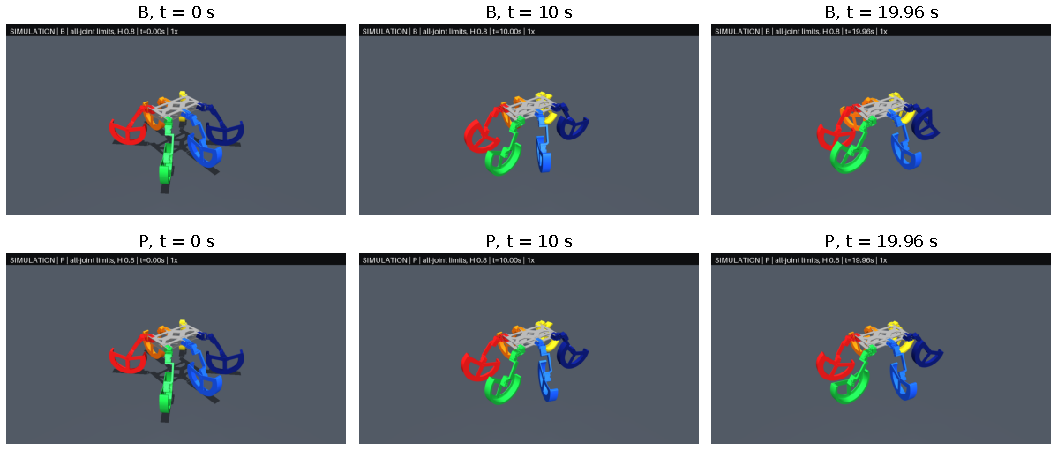
\includegraphics[width=.97\textwidth]{joint_replay.pdf}
\caption{Independent visual replays of B (top) and P (bottom) under H at $\rho=0.8$, phase $1/16$, and a 0.45 m/s forward command. Columns show measurement times 0, 10, and 19.96 s. The camera follows the robot; numerical speed comes from model state. Replayed metrics match their original trial records. These are simulation images, not hardware validation.}
\label{fig:replay}\end{figure*}

\section{DISCUSSION}
\subsection{What the Evidence Supports}
The rewind budget reduces a component of target demand without materially reducing transport in the baseline study. G demonstrates why a distance bound without timely reindexing can make the residual articulated trajectory unreachable. N measures the contribution of rolling within this gait family; it is not an optimized external walking baseline.

The added governor closes the issued-target-rate gap, but does not make B preferable to P. Periodic P remains a strong simpler choice in the evaluated conditions. Moreover, F produces faster transport than H while changing the desired target sequence. A claim that preserving every requested target is necessary for useful locomotion would therefore be unsupported. The main transferable result is the coupling between rewind time, residual travel, and target issuance, including the cost of enforcing each constraint.

\subsection{Remaining Validation Gaps}
A no-load speed is not a loaded actuator capability. The bounds proved here apply to issued targets and internal profiles; the observed actual joint-rate overshoot, tracking errors, and intermittent loaded support require dynamic and contact constraints before a physical feasibility claim. The planner does not constrain acceleration or optimize contact forces.

The model uses rigid tires, disables most link and motor collision geoms, and omits hinge hard stops. A preserved arc cavity does not establish compliant contact or collision clearance. The new 20--60 s runs and command sequences extend the earlier evidence, but do not establish terrain generalization or long-term reliability. Timestep sensitivity must be reported for the constrained study itself.

Archival physical images and the historical stair sequence document embodiment under an earlier, undocumented controller. They lack synchronized logs for B and cannot validate it. The decisive remaining work is loaded actuator identification and matched U/B/P hardware trials with external pose, joint, current, and timing measurements. A direct comparison with a dynamics-aware joint-constrained planner is also needed to establish a broader advantage.

\section{CONCLUSION}
We coupled a finite arc's available rewind time to rolling allocation and residual articulated travel. The baseline study supports reduced sector demand, while the additional all-joint study establishes bounded target issuance and quantifies the effects of gait retiming. Periodic reindexing remains competitive, and rate-limited targets do not guarantee physical joint or contact feasibility. These distinctions define the mechanism's demonstrated scope and the next validation requirements.

\noindent\begin{minipage}{\columnwidth}
\section*{ACKNOWLEDGMENT OF AI ASSISTANCE}
OpenAI Codex assisted with the Abstract, Sections I--VIII, source analysis, controller and evaluation code, and figure and video assembly. Numerical observations came from executed simulations or geometry calculations; physical images came from archival recordings. Generated material was checked against recorded results, source files, and cited sources during manuscript preparation.
\end{minipage}
\par\interlinepenalty=10000
\IEEEtriggeratref{11}\bibliographystyle{IEEEtran}\bibliography{references}
\end{document}
